\section{成像模型}
	针孔模相机成像方式是场景通过相机光心(小孔)在感光元件下留下像,小孔太小会导致成像清晰但暗淡,太大则导致明亮而模糊,对此在小孔前加个凸透镜汇聚光线,使得成像清晰而明亮\footnote{\url{https://en.wikipedia.org/wiki/Pinhole_camera_model}}。

	\begin{figure}[H]
		\begin{center}
			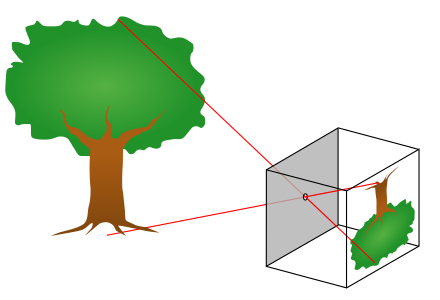
\includegraphics[width=0.48\textwidth]{../images/pinhole.png}
			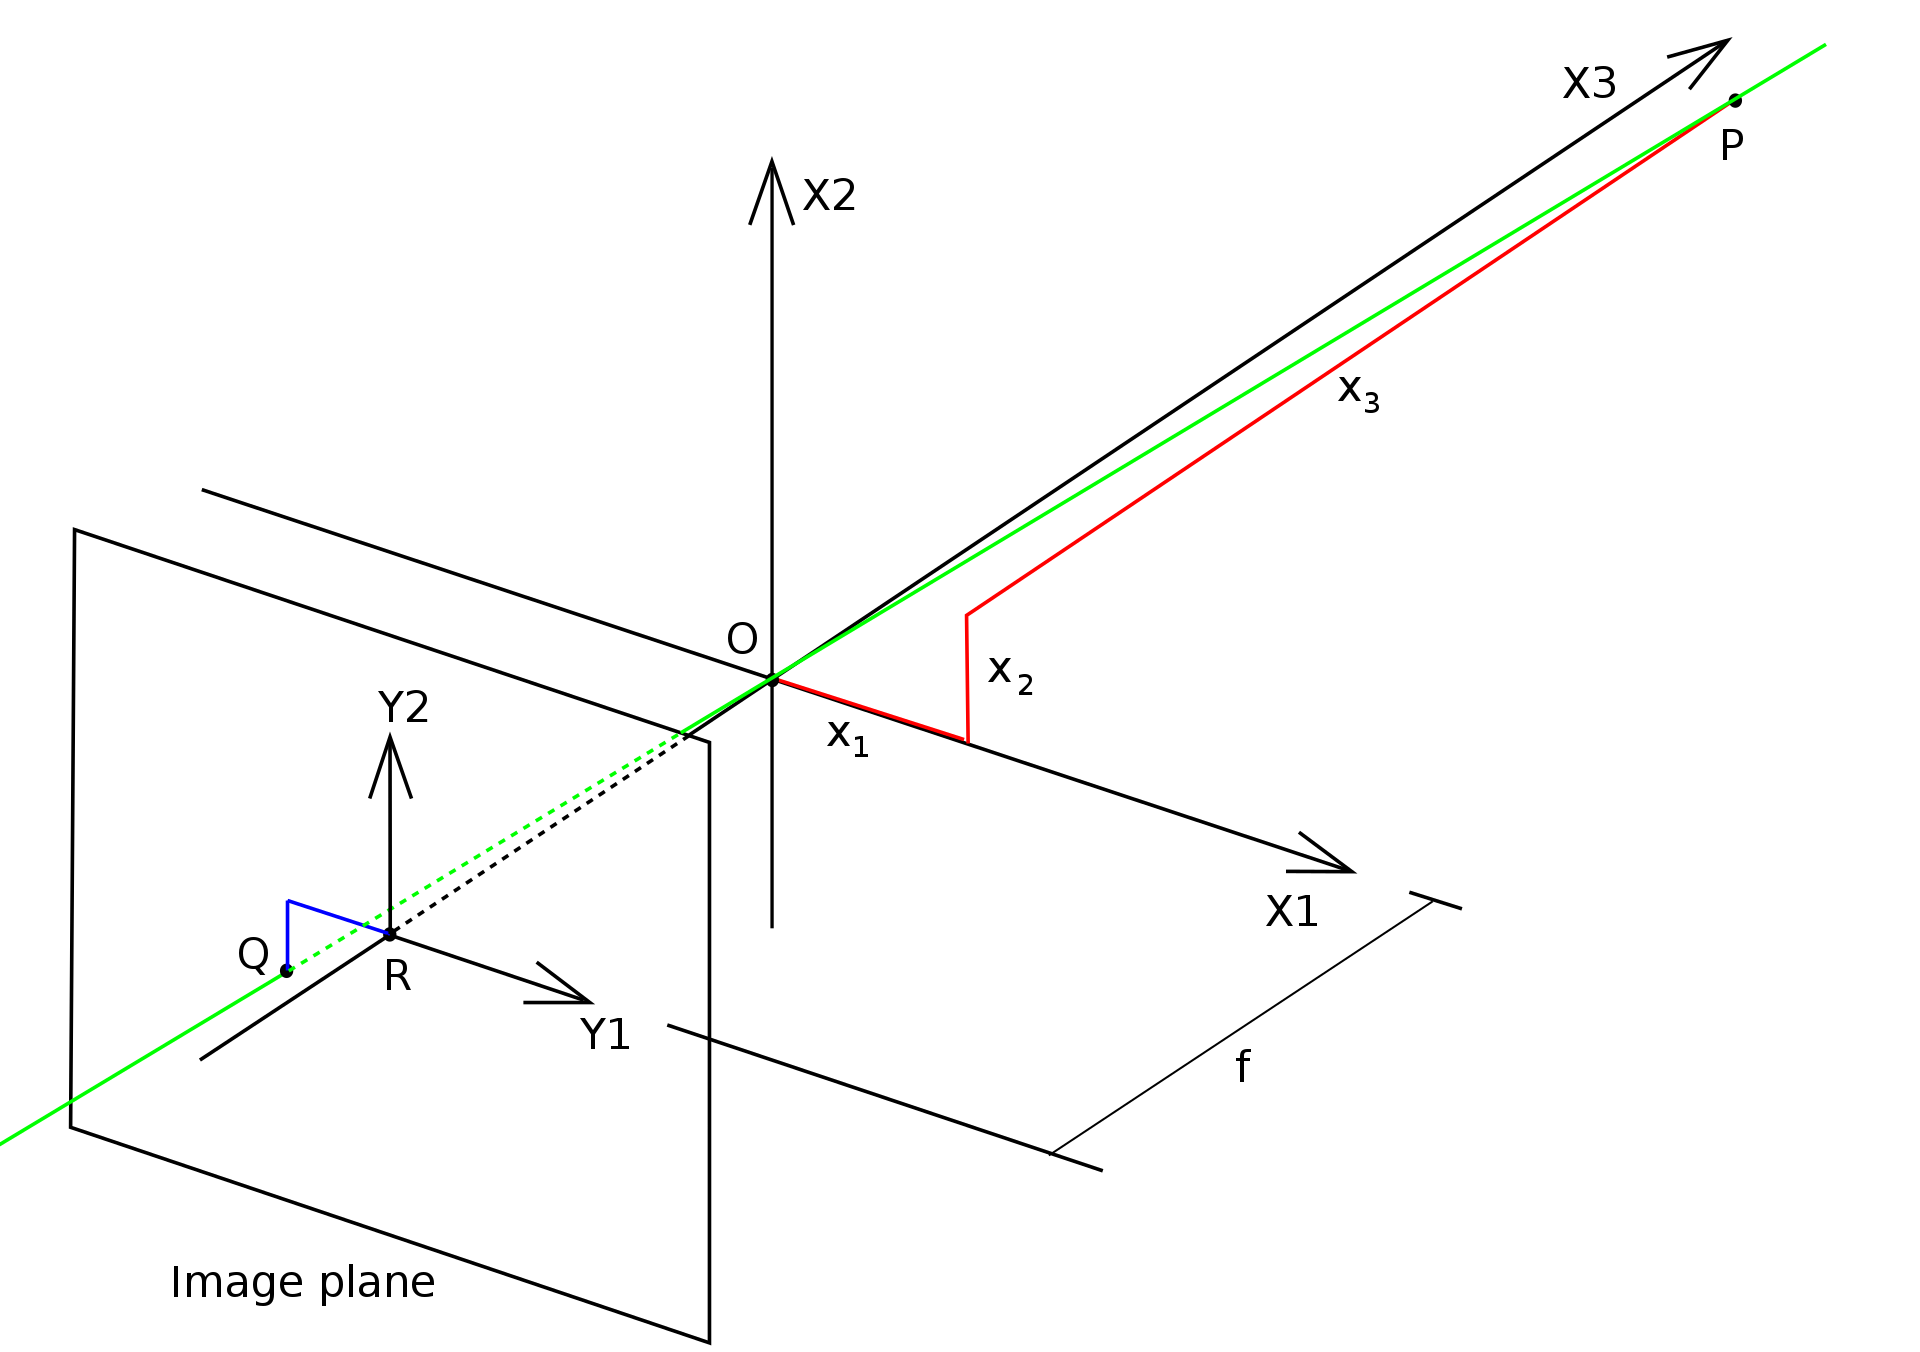
\includegraphics[width=0.48\textwidth]{../images/pinhole_coor.png}
		\end{center}
		\caption{成像模型及相机坐标系}
	\end{figure}

	小孔成像又称为透视成像,当我们拍摄平行铁轨时,照片上铁轨不再平行,并且呈近大远小的特点,这是透视成像的典型特点。\\

	成像过程是一个把空间点投影到像素平面的过程:空间点$P=(x,y,z)$,根据平面几何可知,对应像素坐标为$p = (xf/z, yf/z) = f/z(x,y)$($f$为相机焦距)。\\
	
	$z$不是常数,所以这不是一个线性变换。如果场景点都位于一张平面上,或者场景的深度远远小于场景到相机的距离,可近似认为所有场景点深度都为$z_0$,此时为线性变换,
	$$
		p = \frac{f}{z_0}(x,y)
	$$

	这样的相机称也为\textbf{弱投影相机}或\textbf{仿射相机}。

\subsection{坐标系}
	一般我们要使用到3个坐标系,

	\subsubsection*{世界坐标系}
		世界坐标系用来测量场景的绝对位置,比如可以把原点设置在故宫大殿的中心,这样所有的场景点都会存在一个绝对坐标。\\

		实际上世界坐标只是为了区分不同相机的姿态,无需指定一个绝对位置,常选择第一个相机为世界坐标系。

	\subsubsection*{相机坐标系}
		用来刻画场景相对相机光心的姿态,以光心为原点,光轴为$z$轴,以指向场景的方向为正向;\\

		$xy$平面平行于成像平面,上为$y$轴,右为$x$轴,$z-y-x$符合右手法则;\\

		不同的相机对相同场景,会在各自坐标系中刻画出不同的姿态,在世界坐标系中,可以明确相机坐标系之间的转换关系,统一场景的唯一表示。

	\subsubsection*{像素坐标系}
		像素坐标系$uv$就是2D成像平面,单位是像素,平行于相机坐标系的$xy$平面。\\

		$uv$坐标系的原点一般在图像的左下角或左上角,而$xy$平面的原点在光心,也即$uv$平面的中心,在像素坐标系光心存在一个偏移量$c_x,c_y$(单位为像素)。\\

		世界坐标系和相机坐标系的单位是m,而像素坐标系的单位是pixel,在投影的时候需要明确转换因子,即当前相机1m等于多少pixel

\subsection{相机内参矩阵}
	在相机坐标系中,场景成像与相机本身参数有关,这些参数称为\textbf{内参数},

	\begin{itemize}
		\item 相机焦距$f$,可以调节成像平面与光心的距离,称为\textbf{物理变焦};焦距大成像大,焦距小成像小
		\item 光心偏移量$c_x,c_y$(单位为像素)
		\item 相机偏斜,因为工艺问题,感光元件构成的像平面不是矩形,存在一个角度$\theta$
		\item $x,y$方向可能存在不同的像素转换因子
	\end{itemize}

	这些参数都考虑进来,得到相机\textbf{内参矩阵} $K$,共有5个自由度,

	\begin{equation}
		K = \begin{bmatrix}
			\alpha \quad& -\alpha\cot\theta        \quad& c_x\\
			0      \quad& \frac{\beta}{\sin\theta} \quad& c_y\\
			0      \quad& 0                        \quad& 1
		\end{bmatrix}
	\end{equation}

	\textit{焦距和转换因子已经融合到$\alpha,\beta$参数中。}

\subsubsection*{焦距}

	若为相机没有偏斜,则内参矩阵会简化为,
	\begin{equation}
		K = \begin{bmatrix}
			f_x 	\quad& 0        \quad& c_x\\
			0		\quad& f_y \quad& c_y\\
			0      \quad& 0                        \quad& 1
		\end{bmatrix}
	\end{equation}

	此时内参矩阵有4个参数,为什会有$f_x,f_y$的区别?\\

	实际上像素坐标系是一个离散值,其坐标代表是在$x,y$方向分别有几个像素,像素为$p_w \times p_h$的矩形,单位为微米($\mu m$)。\\

	像素坐标实际是指,
	$$
		f_x = \frac{f}{p_w}, f_x = \frac{f}{p_h}
	$$

	$f$是相机中的焦距,是指成像平面与透镜的距离,单位为$mm$,考虑到单位换算,$1mm = 1000\mu m$,内参矩阵中的焦距计算为,
	$$
		f_x = \frac{1000f}{p_w}, f_x = \frac{1000f}{p_h}
	$$

	针对相机拍摄的照片,可以通过EXIF信息读取拍摄物理焦距($mm$),再查询相机参数,确认像素大小,从而计算出内参矩阵。

\subsubsection*{35mm等效焦距}

	EXIF信息中经常出现两个焦距,一个是拍摄照片时的物理焦距,一个是“等效35mm焦距”。\\

	焦距控制着成像大小,但成像大小还受限于相机感光元件的大小,只有在感光元件相同大小时,讨论焦距之间的大小才有意义,所以经常把不同相机的感光元件对其到某一固定尺寸,即35mm大小。\\

	当年电影之父奥斯卡第一次把35mm高的电影胶片用于他发明的徕卡相机,而电影胶片上下有孔,所以有效高度是24mm,胶片的实际感光面积是$36mm \times 24mm$,并逐渐形成了标准\footnote{\url{https://blog.csdn.net/xback_shaohan/article/details/129771692}}。\\

	“35mm等效焦距”是指保持成像大小不变,感光元件对齐到$36mm \times 24mm$时,对应的焦距。\\

	如果知道了图像分辨率$w \times h$和“35mm等效焦距”,也可计算出内存矩阵中的焦距\footnote{\url{https://www.reddit.com/r/computervision/comments/dch9xz/alculate_camera_intrinsics_focal_lengths_from/?rdt=51846}},
	$$
		f_x = w * focal\_equal\_35mm/36, f_y = h * focal\_equal\_35mm/24
	$$

\subsubsection*{FOV}
	还经常讨论相机另一个指标,\textbf{视场}(FOV, Field Of View),是指相机焦点与感光元件的夹角,具体有三个,
	\begin{itemize}
		\item \textbf{HFOV},水平夹角$\alpha$
		\item \textbf{VFOV},竖直夹角$\beta$
		\item \textbf{DFOV},对角线夹角$\gamma$
	\end{itemize}

	感光元件大小为$w,h$,容易知道,
	\begin{align*}
		\tan\frac{\alpha}{2} &= \frac{w}{2f_{pixel}}\\
		\tan\frac{\beta}{2} &= \frac{h}{2f_{pixel}}\\
		\tan\frac{\gamma}{2} &= \frac{\sqrt{w^2 + h^2}}{2f_{pixel}}\\
	\end{align*}

	所以,只要知道了图像宽高也容易计算出$f_{pixel}$。\\

	比如说,相机对角视角为$77.7^\circ$,图像分辨率是$4032 \times 3024$ pixels,则对角线有5040 pixels,对角焦距为\footnote{\url{https://stackoverflow.com/questions/69159247/camera-calibration-focal-length-value-seems-too-large}},
	\begin{align*}
		f &= (5040/2)\tan(77.7/2)\\
		f &= 3128.6
	\end{align*}

\subsubsection*{相机投影}
	相机坐标系点$P$,在像素平面的投影为,

	$$
		P^{\prime}  = KP
	$$

	上面得到的$P^{\prime}$是2D平面的齐次坐标,转换为2D坐标还需,
	$$
		p = \left(\frac{K_1P}{K_3P}, \frac{K_2P}{K_3P}\right)^T
	$$
	$K_1,K_2,K_3$是$K$的行向量。\\

	对任意尺度因子$d$($d\neq 0$),$dP$为经过光心和$P$的射线,投影像素坐标为,
	$$
		p_d = p
	$$

	这说明射线上所有的点都投影到相同像素上,相机投影实际就是一个降维的过程。\\

	反之,已知像素平面上一点$p$(齐次坐标),反投影到3D空间会得到一条射线,

	\begin{equation}
		P(d) = dK^{-1}p \label{inverse_proj}
	\end{equation}

	如果知道两张图像中点两个的对应关系,则通过反向投影,二者的交点,即为对应空间点的坐标。\\

	如此确定3D点坐标似乎很简单,然而实际并不可行,因为在噪音的影响下,空间中两条直线很难相交,实际需用\textbf{三角化}的方法求解。

\subsection{相机投影矩阵}
	内参矩阵刻画场景在相机坐标系下的投影关系,如果场景在世界坐标系下,需要把场景从世界坐标系通过旋转平移变换到相机坐标系,再用内参矩阵进行投影。
	$$
		M = K\left[R\quad T\right]
	$$

	$R,T$为相机坐标系的旋转矩阵和平移向量,$\left[R\quad T\right]$称为相机\textbf{外参矩阵},$M$称为相机的\textbf{投影矩阵}。\\

	投影矩阵是内参矩阵乘以外参矩阵,是一个$3\times 4$的矩阵。\\

	也可以对投影矩阵增广到$4\times 4$的矩阵$\tilde{M}$,

	$$
		\tilde{M} = \begin{bmatrix}
			KR\quad& KT\\
			0\quad& 1
		\end{bmatrix}
	$$

	$\tilde{M}P$投影得到一个$4\times 1$的向量,在代数上这个向量前3维代表像素的齐次坐标,但在几何上没有意义。\\

	增广矩阵主要是能在反投影时简化计算,后面会用到。

\subsection{三角化}
	如果知道两张图像中两个点$p_1,p_2$的对应关系,根据投影矩阵可知,
	\begin{align*}
		p_1 &= M_1 X\\
		p_2 &= M_2 X\\
	\end{align*}

	对应像素坐标为,
	\begin{align*}
		u_1 = \frac{m_{11} X}{m_{13} X}, \quad v_1 = \frac{m_{12} X}{m_{13} X},\quad
		u_2 = \frac{m_{21} X}{m_{23} X}, \quad v_2 = \frac{m_{22} X}{m_{23} X}
	\end{align*}

	整理成齐次方程,
	$$
		\begin{bmatrix*}
			&u_1m_{13} - m_{11}\\
			&v_1m_{13} - m_{12}\\
			&u_2m_{23} - m_{21}\\
			&v_2m_{23} - m_{22}\\
		\end{bmatrix*} X = 0
	$$

	提供一对匹配点有4个方程,$X$是一个三维向量,所以通过奇异值分解能快速求解3D坐标,这个方法称为\textbf{三角化}。